\documentclass[%
 reprint,
%superscriptaddress,
%groupedaddress,
%unsortedaddress,
%runinaddress,
%frontmatterverbose, 
%preprint,
%preprintnumbers,
%nofootinbib,
%nobibnotes,
%bibnotes,
 amsmath,amssymb,
 aps,
%pra,
%prb,
%rmp,
%prstab,
%prstper,
%floatfix,
]{revtex4-2}

\usepackage{graphicx}% Include figure files
\usepackage{subcaption}
% \usepackage{subfigure}

\usepackage{dcolumn}% Align table columns on decimal point
\usepackage{bm}% bold math
%\usepackage{hyperref}% add hypertext capabilities
%\usepackage[mathlines]{lineno}% Enable numbering of text and display math
%\linenumbers\relax % Commence numbering lines

%\usepackage[showframe,%Uncomment any one of the following lines to test 
%%scale=0.7, marginratio={1:1, 2:3}, ignoreall,% default settings
%%text={7in,10in},centering,
%%margin=1.5in,
%%total={6.5in,8.75in}, top=1.2in, left=0.9in, includefoot,
%%height=10in,a5paper,hmargin={3cm,0.8in},
%]{geometry}

% Fix excessive list spacing in REVTeX
\usepackage{paralist}
\setdefaultleftmargin{2em}{}{}{}{}{}

\newcommand{\greekfi}{Greek.fi }


\begin{document}

\title{\greekfi - Decentralized American-Style Options Protocol}

\author{Mahmoud Lababidi}
\email{ml@greek.fi}
\affiliation{%
\greekfi 
}

\date{June 26, 2025}

\begin{abstract}
\greekfi is a protocol that enables decentralized American-style exercise options that are fully collateralized without requiring oracles or margin. 
It is designed for composability, exercisability, and universal use on any EVM-compatible chain and allows any ERC20 token to be used as collateral and consideration, including WBTC, WETH, stETH, USDC, and USDT. 

Similar to yield generating tokens, the protocol generates two ERC20 tokens: a redemption token (which provides capital efficiency) and an option token.
We dive into the mechanics of these tokens and how they impact a new level of composability to create a new options ecosystem that both encompasses and surpasses traditional financial options strategies.


\end{abstract}

\maketitle

\section{Introduction}

\subsection{Background}
Options in crypto have exploded recently in usage and types of approaches. 
Across 24-hour averages, over \$6B of trading volume occurs in perpetual markets. 
In addition, Deribit was recently purchased by Coinbase for nearly \$3B. 
This is unsurprising and can see a ramp-up to catch up to the traditional finance market as the traditional finance market sees \$2.7T USD in daily notional trading in the options market and \$600B in daily open interest. 

The DeFi space still has room to grow but one issue may be holding it back from growth: early exercisable (American) options do not exist in a liquid, decentralized, tokenized manner which will allow options to become as commonplace in the DeFi ecosystem as yield generating tokens. 
Early exercise is an added benefit in options because it gives in-the-money holders an incentive to exercise early.

To solve this, we introduce the \greekfi protocol, the first fully decentralized, collateralized, tokenized, exercisable, expirable options protocol in the Ethereum ecosystem.
The protocol achieves the following, which fulfill the requirements for an American options:
\begin{itemize}
  \setlength{\itemsep}{0pt}
  \setlength{\parskip}{0pt}
  \item Fully ERC20 compatible - allowing full composability
  \item Fully collateralized protocol so that every option can be exercised to swap for the collateral
  \item Exercisable so that the option holder can swap consideration tokens for the collateral
  \item The option writer can redeem consideration prior to expiration
  \item The option writer can redeem collateral post expiration
  \item The option writer can redeem collateral prior to expiration if they also own the option
  \item Two tokens/contracts drive the protocol (LONG and SHORT) similar to yield platforms
  \item Oracle-free, margin-free
\end{itemize}

This protocol will unlock a trove of possibilities to DeFi, for example:

\begin{itemize}
  \setlength{\itemsep}{0pt}
  \setlength{\parskip}{0pt}
  \item Hedge short-term and long-term risk as well as take on risk
  \item Use leverage without getting margin called
  \item Earn yield through covered calls
  \item Create exotic options strategies
  \item Create unique underlying swap pairs beyond USD bases
  \item Transfer options from within ecosystems to other ecosystems
  \item Trade options in both OTC and other markets
  \item Cash Settlement through flash-loans
\end{itemize}

\section{Protocol Overview}

The \greekfi protocol uses a contract factory, allowing upgradability, which creates a new pair (SHORT and LONG) of ERC20 contracts/tokens for each option type created (i.e. WETH/USDC, WBTC/USDC).
The pair token creation provides ERC20 composability in SHORT and LONG, a necessity in the adoption of options as tokens.
The pair provides a minting interface where depositing collateral tokens returns SHORT and LONG tokens.
Each option pair is represented by a tuple of the following parameters:
\begin{equation*}
  (Collateral, Consideration, Strike, Expiration, isPut).
\end{equation*}

In Options, Collateral is the underlying asset that the option holder has the right to purchase, while Consideration is the asset paid in exchange for the Collateral. They are both represented by contract addresses.
The Expiration is the last date the option can be exercised. 
It is represented as a Unix timestamp, similar to block timestamps.
The Strike is the price at which the option can be exercised.
The Strike is represented as a ratio of the Consideration to the Collateral with an additional temporary multiplier of $10^{18}$ as a buffer since solidity does not support decimals.
The boolean, isPut, indicates if the option is a Put option, which is only for vanity. 
This protocol allows the collateral and consideration to be any ERC20 asset, meaning USDC and WETH could be collateral/consideration or consideration/collateral. 
This flexibility removes any special complications of Put options. 
Only the front end handles inverting the Strike price for the user (i.e., 1000 USDC for 1 WETH is represented as 1 USDC for .0001 WETH). This is similar to how Swapping platforms visualize the price, where it is inverted when clicked. In the future, there may be a way to automatically determine if a pair is considered a Put or Call, but a puzzle to the reader, is WETH/WBTC a call or a put?
\begin{figure}[h]
  \centering
  \begin{subfigure}[b]{0.45\textwidth}
    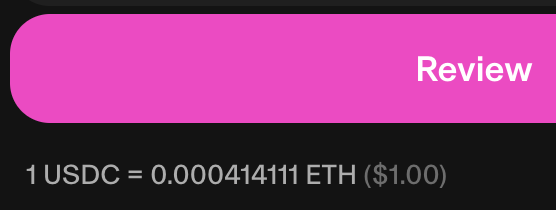
\includegraphics[width=\textwidth]{swap1.png}
    \caption{Swap 1}
    \label{fig:swap1}
  \end{subfigure}
  \hfill
  \begin{subfigure}[b]{0.45\textwidth}
    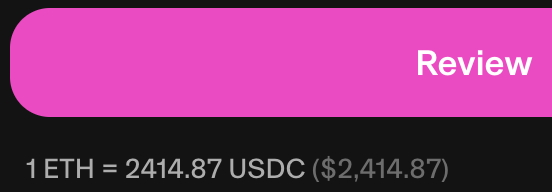
\includegraphics[width=\textwidth]{swap2.png}
    \caption{Swap 2}
    \label{fig:swap2}
  \end{subfigure}
  \caption{Swap diagrams}
  \label{fig:swaps}
\end{figure}


The LONG and SHORT contracts are coupled to each other, meaning every interaction with the LONG token will interact with the SHORT token.
The proper movement of collateral and consideration through exercise and redemption is heavily dependent on this coupling.

The diagram below is a visual representation of an exercise, a coupled process. 
In order to exercise the SHORT option, the user's consideration is swapped for the collateral held by the SHORT contract.
\begin{figure}[h]
  \centering
  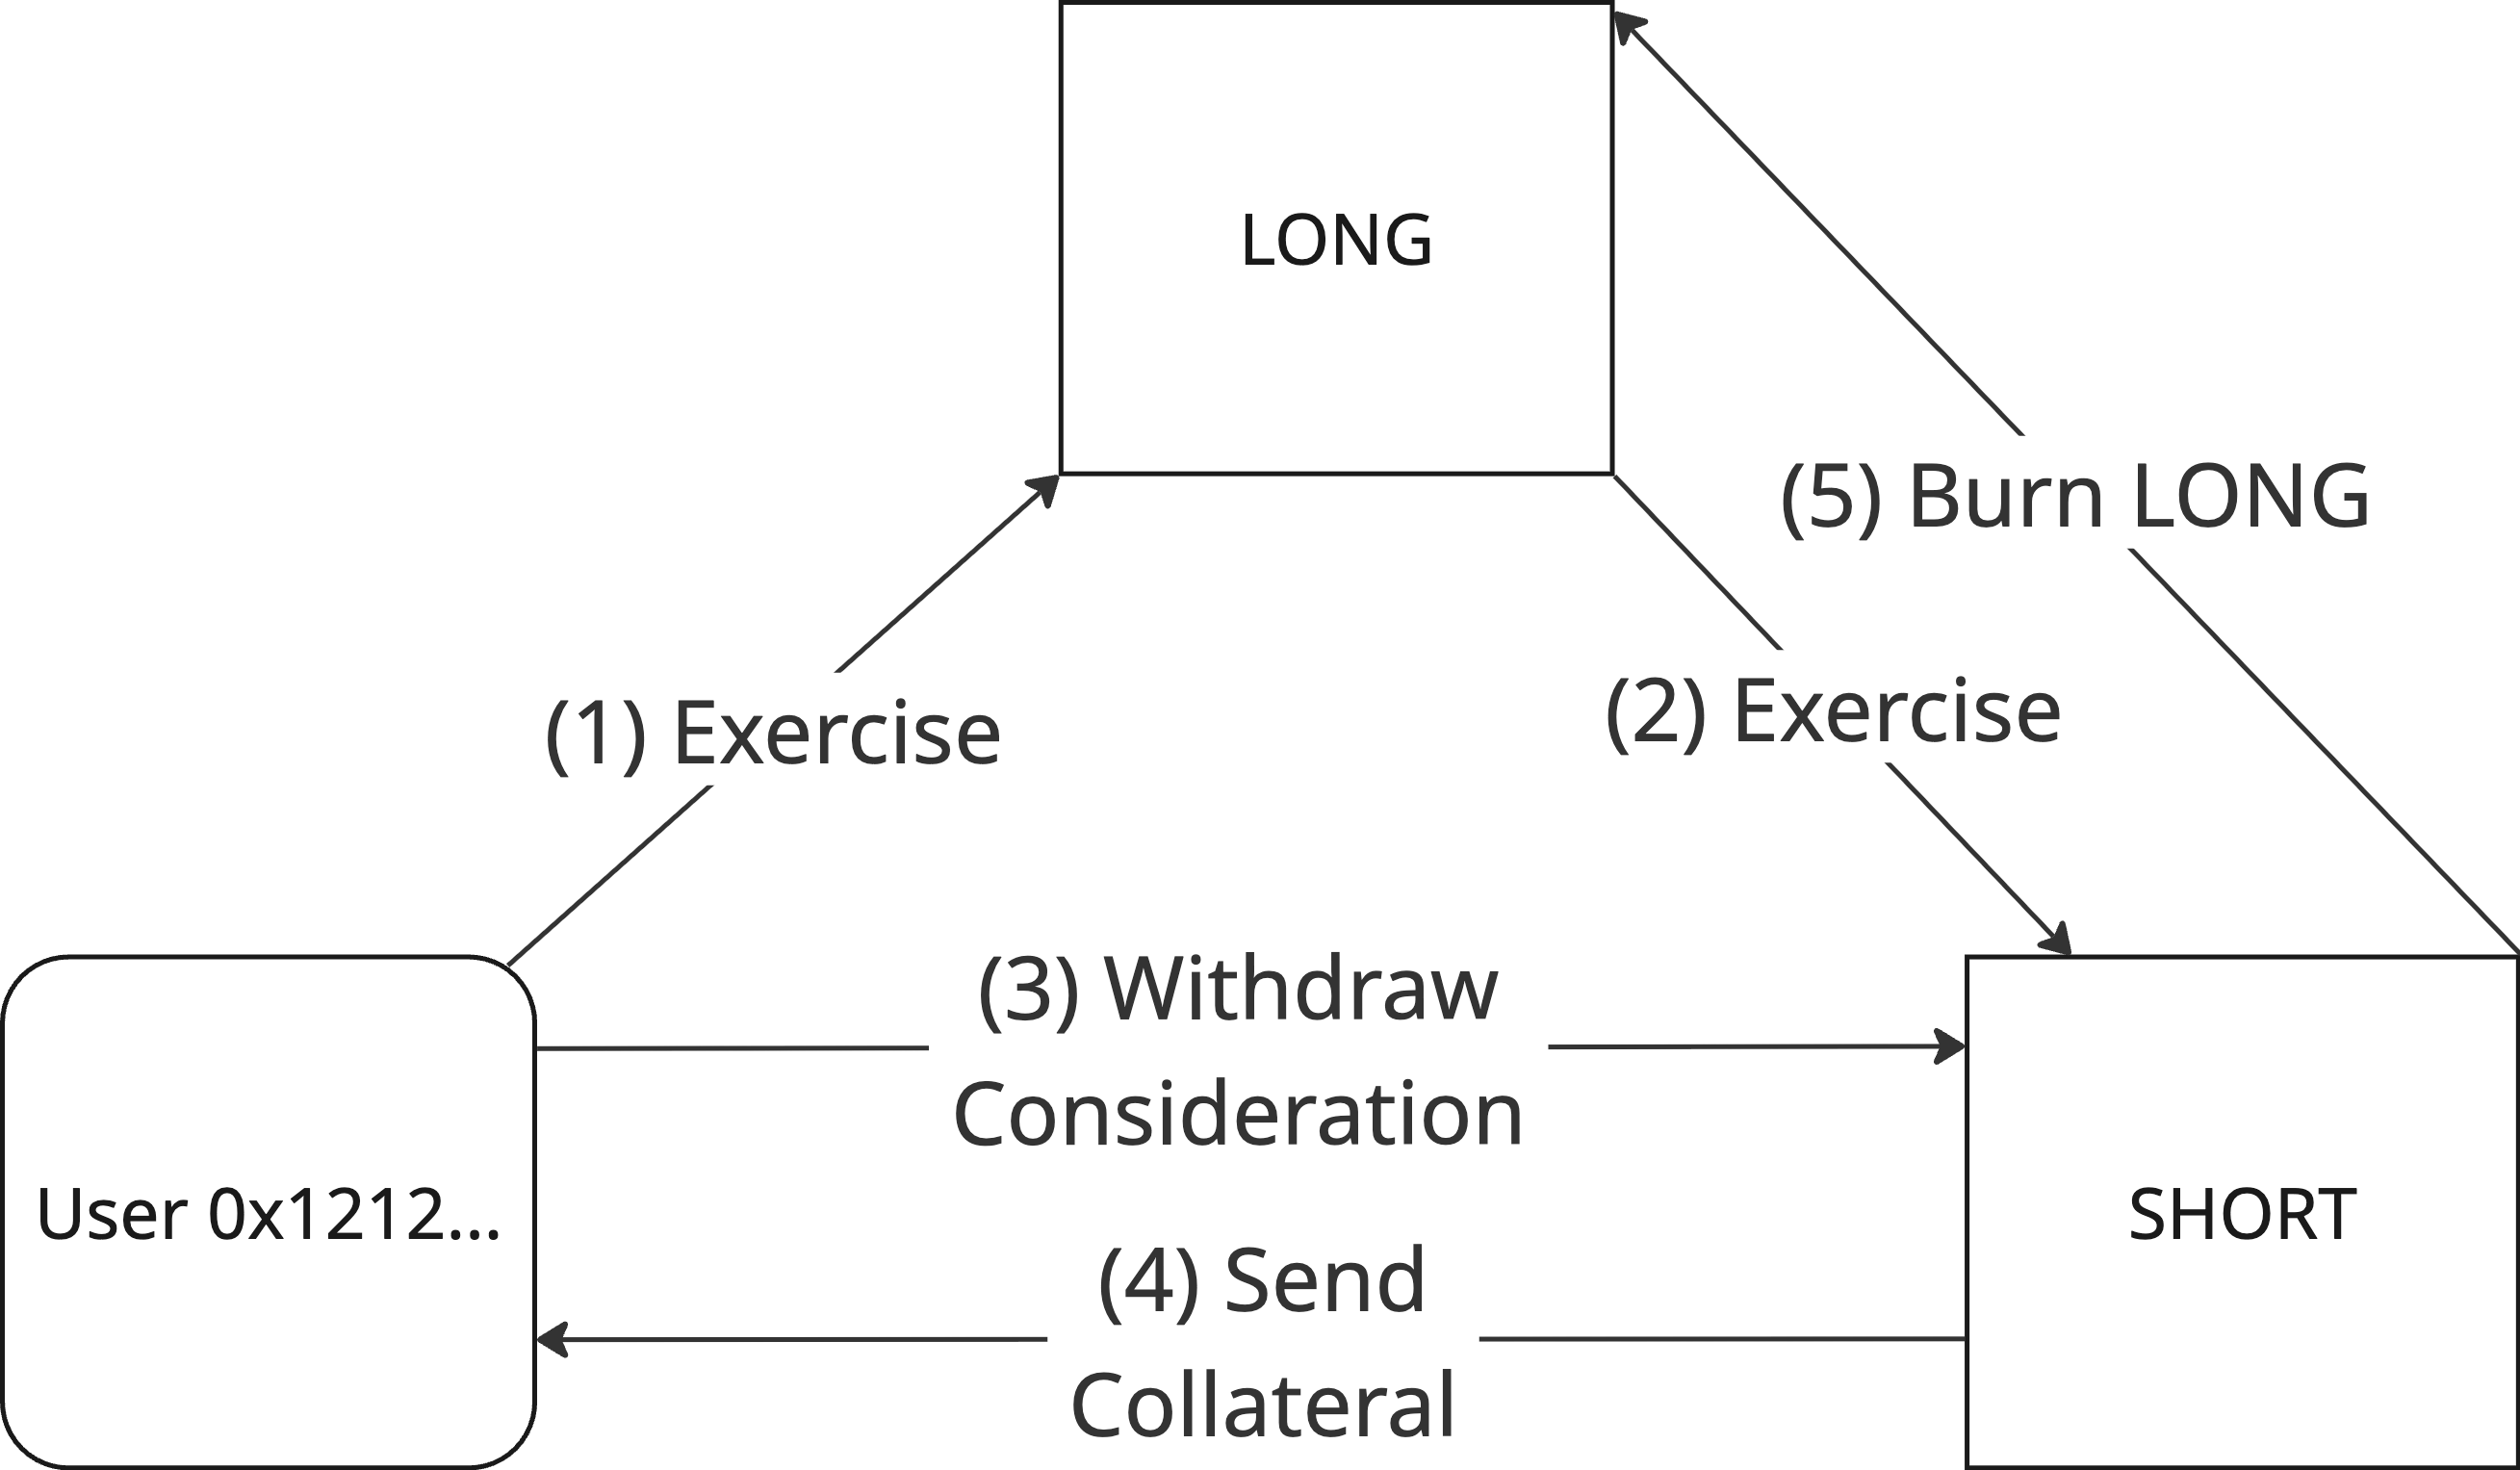
\includegraphics[width=0.5\textwidth]{exercise.png}
  \caption{Diagram of the steps to exercise the option}
  \label{fig:exercise}
\end{figure}

\subsection{LONG Token}

The LONG token represents the long position of the option holder,
entitled to purchase the underlying collateral asset when exercising the option. 
Simply put, the LONG token is the so-called "Option" in the traditional options world.

The LONG token can only be exercised before expiration. After expiration, the LONG token 
is unusable and deemed worthless. We leave room to burn expired tokens so they aren't used for scams. 

The LONG token can be traded on DEXs/AMMs and traded on RFQs. 
They can also be used for OTC trades between private parties.

Other than standard ERC20 functionality, the LONG token permits a user to \textbf{exercise} the option and 
\textbf{redeem} the underlying collateral if and only if they hold the SHORT token as well. 
The \textbf{lock} and \textbf{unlock} functions are also available to prevent and allow exercise - this feature is for vesting or credit default swaps.

\begin{table}[h]
\centering
\begin{tabular}{|p{3cm}|p{4cm}|}
\hline
\textbf{Function} & \textbf{Description} \\
\hline
mint()  & Mints LONG and SHORT tokens by depositing collateral. \\
\hline
exercise() & Exercises the option by swapping consideration for collateral. \\
\hline
redeem() & Redeems collateral before expiration if also holding LONG. \\
\hline
lock()/unlock() & Locks/unlocks to prevent/allow exercise. \\
\hline
\end{tabular}
\caption{Available functions for LONG token}
\label{tab:functions}
\end{table}


\subsection{SHORT Token}

The SHORT token represents the short position of the option writer,
obligated to sell the underlying collateral asset for the consideration
asset when the LONG option is exercised. 
In TradFi, when an option is written and sold, the account shows a negative balance of the option. 
We represent this position with the SHORT token. 

\paragraph*{SHORT is Put?} The SHORT token is not a Put option. It is a short position in the option trade. 
Being short does represent an expected negative outlook on the Collateral asset wrt the Consideration asset, 
which is similar to a Put option but they are not the same.



The SHORT token also represents a long position in the underlying Collateral asset by locking up the underlying collateral asset in the SHORT token.
This token structure not only represents a covered call, but is the only way to provide the ability to exercise the protocol.
This is the first step to providing a fully collateralized protocol.
The SHORT token is also able to redeem the underlying collateral asset after expiration.

The SHORT token provides an ability to redeem the underlying collateral asset after expiration.
Additionally, prior to expiration, the SHORT token provides the ability to redeem the consideration asset after LONG holders exercise.
And finally, if a SHORT holder also owns the LONG token, they can redeem the collateral prior to expiration (this is gamma neutral).

\begin{table}[h]
\centering
\begin{tabular}{|p{4cm}|p{4cm}|}
\hline
\textbf{Function} & \textbf{Description} \\
\hline
redeem() & Redeems collateral after expiration. \\
\hline
redeemConsideration() & Redeems consideration if available. \\ 
\hline
\end{tabular}
\caption{Available functions for SHORT token}
\label{tab:functions}
\end{table}


\subsection{Capital Efficiency}

At this point, one may wonder about the capital efficiency (CE) of the protocol. 
This requires a couple of additional pieces to be added outside of the protocol.
One requirement for CE is for the SHORT token to be used as collateral for loans for the underlying asset.
Lending protocols are willing to lend against an asset if a few conditions are met. 
The two that are not very clear in this protocol are:
\begin{itemize}
  \setlength{\itemsep}{0pt}
  \setlength{\parskip}{0pt}
  \item The asset has a market, i.e., is liquid
  \item The asset has a price feed, i.e., an oracle
\end{itemize}


To clarify, the protocol has no Oracle included and no margin ability. 
Many protocols use margin and use cash settling to settle the option.
This prevents the ability to exercise the option and gain collateral.

This protocol presents a few interesting challenges to price feeds and liquidity. 
Firstly, liquidity is a necessity so that the lending protocol can sell the asset in the case of a margin call.
Secondly, a price feed is necessary to determine if the loan is at risk of being called.

If the lending protocol restricts the loan to provide only the underlying collateral or the consideration asset,
the lenders have two regimes of the price of the Collateral to consider: 
when the price of the collateral is above the strike price, and when the price of the collateral is below the strike price.
Below Strike (K), SHORT is worth P, the price of the collateral. 
Above Strike (K), SHORT is worth only K because the consideration has been paid through exercise.
The chart below shows the price of the SHORT token in those regimes with a Strike of 3000.
\begin{figure}[h]
  \centering
  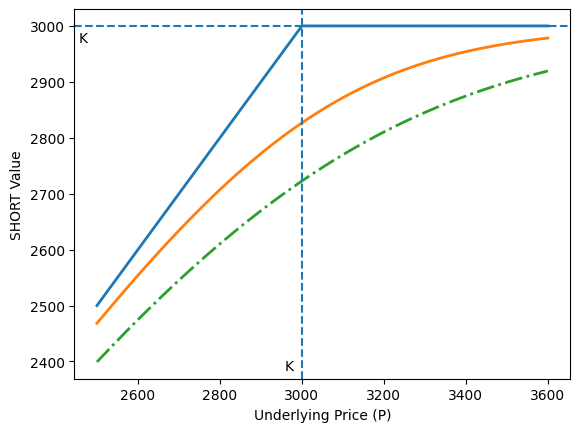
\includegraphics[width=0.5\textwidth]{short_price.png}
  \caption{Price of the SHORT token in the two regimes. The orange solid line shows the realistic price incorporating LONG token value, while the green dot-dashed line shows an extreme fair price for low-volume assets.}
  \label{fig:short_price}
\end{figure}

The combination of the two regimes is not linear and the price feed needs to provide a version of this non-linearity or the lender needs to account for it.
More importantly, the more realistic price of the SHORT token incorporates the market price of the LONG token, as seen as the orange curve solid line in the chart above.
Again, another consideration for the oracle, but for assets that have low volume, an extreme fair price can be used by really shifting the LONG token price component as seen by the green dot-dashed line in the chart above.

\paragraph*{Margin Call Mechanics}
If the lender needs to margin call against the SHORT token, there are two options: 1. The Lender can buy the coupled LONG token, redeem the resulting collateral and either swap it or use it to pay back the loan. 2. If there's a liquid market for the SHORT token, immediately sell it to cover the loan, with a possibility of using the proceeds to buy the borrowed collateral.

\subsection{Fees}
The protocol reserves the possibility of fees in the future at various places related to the protocol.
Anything around 1 bip would be considered, with a tapering ($\log(volume)$) to incentivize large volumes.
\begin{itemize}
  \setlength{\itemsep}{0pt}
  \setlength{\parskip}{0pt}
  \item Protocol fee, where anything around 1 bip on minted options would be considered.
  \item AMM fee, where a revenue share would be split with Liquidity Providers.
  \item Exercise fee, where a fee would be charged on the exercise of the option.
  \item Vault fee, where a fee would be charged for the vault management.
\end{itemize}


\section{Applications and Future Considerations}
\paragraph*{AMM}
The protocol tokens can be used in an AMM, thus creating a market for the options, as well as the short positions if desired. 

\paragraph*{Default Swaps}

The protocol is able to provide default swaps as insurance for risk management in debt markets. 
An Oracle or Third party can \textbf{unlock} the LONG token to allow exercise.

\paragraph*{Cash Settlement}
If stock settlement/exercise feature is not really needed in the space and margin is desired, 
then the composable nature of the protocol can be used to create a margin protocol through the mechanics described above. 


\paragraph*{Interoperability across chains}

In the context of the Optimism Superchain, we leave room for the protocol to handle an ability to be interacted with across chains.
This means that exercising will involve movement of collateral and consideration across chains.
There's no free lunch with the interop, but the protocol can be upgraded to handle this with careful design.

\paragraph*{Option Drops instead of Token drops}
In TradFi, options are vested by startup employees and exercised for tax purposes.
A similar use case can be made here to provide option drops instead of token drops.

\paragraph*{Compound Options}
A compound option is an option on an option. Yes, this is a thing. It's basically a second derivative.
And yes, this protocol can handle it. 

\paragraph*{Trading}

Once options are minted, the obvious question is how to trade them. We
have considered using a DEX AMM, such as Uniswap, but options could have
low volume and low liquidity. This can cause slippage and nobody wants
that.

The obvious solution is to use RFQs, such as 0x, Bebop, etc. This allows
for the options to be traded at a price that is determined by the
market. This would allow partnering with market makers to provide
liquidity for the options. This would also solve pricing the options
where the MMs set their own prices. This will create a new market maker
ecosystem.

\paragraph*{Short Token Trading}

The SHORT token represents two things:
Collateral/consideration ownership and a short position in the option
trade. Let's say you sold an in the money call (WETH at 3000 expiring
soon). When you sold your LONG token you received a premium of 1000 USDC
in addition to IV and Time Value. This is potentially priced in the
SHORT token making it tradable since it has a value.

\paragraph*{Vaults}

Vaults allow for more complex strategies using the options protocol.
This simplifies the experience for users and reduces the amount of work
required to implement these strategies.

\paragraph*{Covered Call Vaults}

One strategy, such as covered call vaults, which allow for the creation
of options with a portion of the collateral as the option premium. A
simple strategy could involve users depositing WETH as collateral, and
then the vault handles:
\begin{enumerate}
\item minting options with the collateral
\item selling the options
\item let the options expire worthless
\item redeem the collateral
\item Go to step 1
\end{enumerate}

This strategy is nearly identical to ETF strategies (i.e., XYLD). Covered
call vaults do not exist on chain, but this protocol allows for the
creation of these strategies. This same strategy can be applied for
Covered Put vaults, where the vault mints the put options and sells
them.

\paragraph*{Margined Options Vaults}

Similar to covered call vaults, margined options vaults allow for the
minting of call options using collateral. Afterwards, the vault takes a
loan on the collateral (AAVE, Silo, etc) and uses the proceeds to mint
more options. This allows for the vault to mint more options than it
would have been able to otherwise. This is also extremely risky as the 
vault is exposed to the risk of the collateral asset price.

\paragraph*{Cash Settled Options} 

Using cash-equivelent from a flash loan, 
a contract can be exercised for collateral which 
in turn is swapped for the original cash equivelent.
This whole process can be wrapped in a separate contract
and triggered by an external party near expiration time.

\section{\label{sec:appendix}Appendix}


\begin{acknowledgments}
We wish to acknowledge the support of the DeFi community in developing
the Greek.fi Protocol, offering suggestions and encouragement, testing new versions,
and providing valuable feedback on the design and implementation.
\end{acknowledgments}

\appendix

\subsection{Key Concepts}

\begin{itemize}
\item
  \textbf{Call Option}: Right to buy an asset at a specified price
  before expiration
\item
  \textbf{Put Option}: Right to sell an asset at a specified price
  before expiration
\item
  \textbf{Strike Price}: The price at which the option can be exercised
\item
  \textbf{Expiration Date}: The last date the option can be exercised
\item
  \textbf{LONG Token}: Represents the right to exercise the option
\item
  \textbf{SHORT Token}: Represents the obligation and right to the
  collateral
\end{itemize}

Options need the following abilities to be considered American style:
\begin{itemize}
  \setlength{\itemsep}{0pt}
  \setlength{\parskip}{0pt}
  \item Expirable at some future fixed date
  \item Exercisable so that the option holder can swap consideration for underlying collateral prior to expiration
  \item The option writer can use the collateral freely after expiration, unless...
  \item The contract written has been exercised, providing consideration to the option writer to be used freely
\end{itemize}

  \section{Example: Minting Options}

  \begin{enumerate}
  \item
    Connect your wallet to the protocol
  \item
    Select option parameters:
    \begin{itemize}
    \item
      Collateral Asset: WETH
    \item
      Consideration Asset: USDC
    \item
      Strike Price: 5000 USDC
    \item
      Expiration Date: 30 days
    \item
      Option Type: Call
    \end{itemize}
  \item
    Mint and approve the LONG contract to capture your WETH
  \item
    Receive LONG and SHORT tokens
  \end{enumerate}
  
% \paragraph*{Ignore below}

% Uniswap is a protocol for automated token exchange on Ethereum. 
% It is designed around ease-of-use, gas efficiency, censorship resistance, and zero rent extraction. 
% It is useful for traders and functions particularily well as a component of other smart contracts which require guaranteed on-chain liquidity.

% Most exchanges maintain an order book and facilitate matches between buyers and sellers. 
% Uniswap smart contracts hold liquidity reserves of various tokens, 
% and trades are executed directly against these reserves. 
% Prices are set automatically using the constant product (x*y=k) market maker mechanism, which keeps overall reserves in relative equilibrium. 
% Reserves are pooled between a network of liquidity providers who supply the system with tokens in exchange for a proportional share of transaction fees.

% An important feature of Uniswap is the utilization of a factory/registry contract that deploys a separate exchange contract for each ERC20 token. These exchange contracts each hold a reserve of ETH and their associated ERC20. This allows trades between the two based on relative supply. Exchange contracts are linked through the registry, allowing for direct ERC20 to ERC20 trades between any tokens using ETH as an itermediary.

% This document outlines the core mechanics and technical details for Uniswap. Some code is simplified for readability. Safety features such as overflow checks and purchase minimums are ommited. The full source code is availible on GitHub.

\end{document}
